This section describes the procedure to use {\sc mixmod} graphical user's interfaces. This procedure is roughly
speaking the same for Scilab and Matlab environments.
The two functions {\em mixmodGraph.sci} (Scilab) and {\em
mixmodGraph.m} (Matlab) are available, in the directory MIXMOD/, to launch {\sc mixmod} graphical
user's interface in Scilab (or Matlab) environment.\\
%After executing {\em initMixmod.sci} Scilab function, or adding {\sc mixmod} path to Matlab path,
%{\sc mixmod} interface can be launched using the following command\\

{\noindent Remark With Scilab, you have to execute {\em initMixmod.sci} and
with Matlab, you have to add {\sc MIXMOD} and {\sc MIXMOD/UTIL/MATLAB} directories to Matlab path before
using {\em mixmodGraph.sci} or {\em mixmodGraph.m}}.

%\begin{tabular}{c|c}
%\begin{minipage}[c]{0.30\columnwidth}%
{\scriptsize
\begin{verbatim}
    -> (>>) mixmodGraph;
\end{verbatim}}
%\end{minipage}%
%&
%\begin{minipage}[c]{0.70\columnwidth}%
%{\scriptsize
%\begin{verbatim}
%    >> mixmodGraph;
%\end{verbatim}}
%\end{minipage}%
%\end{tabular}\\

\noindent{Once {\sc mixmod} is launched, the {\em Main Menu} window appears. It contains
the four following choices}
\begin{itemize}
  \item {\em Discriminant Analysis}, to start discriminant analysis,
  \item {\em Cluster Analysis} (or density estimation), to start cluster analysis,
  \item {\em Demos}, to start demonstration session,
  \item {\em Settings} (only for Scilab), to change the display mode,
  \item {\em Help}, provides further information on {\sc mixmod} software.
\end{itemize}

%-----------------------
%-----------------------
\subsection{Demo menu}
%-----------------------
%-----------------------
We propose to begin by a demonstration session. A first contact
with {\sc mixmod} can be made by clicking on {\em Demos} in {\em Main Menu} and,
selecting a data set example, for instance Birds.% and Old Faithfull Geyser.

%---------------------------------------------------------------
\subsubsection{Example with Birds data set}
%---------------------------------------------------------------
\begin{figure}[!hb]
  \centering
  \includegraphics[width=5.5cm, height=4.5cm]{birds.eps}
  \caption{Birds demonstration: multinomial distribution with three components (general model $[Binary\_{p_k}\_{E_{kjh}}]$ see Table \ref{10models}).}
\end{figure}

%\newpage

%-----------------------------------------------------------------------
%\subsubsection{Example with Old Faithfull Geyser data set}
%See \ref{geyserFig1}.
%-----------------------------------------------------------------------
\begin{figure}[!h]
  \centering
  \includegraphics[width=5.5cm, height=4.5cm]{geyser1.eps}
  \caption{Old Faithful Geyser demonstration: Gaussian mixture model with two components (general model $[p_k\lambda_kC]$ see Table \ref{28models}).}
  \label{geyserFig1}
\end{figure}

%--------------------------------
%--------------------------------
\subsection{Cluster analysis}
%--------------------------------
%--------------------------------

%-------------------------------------------
\subsubsection{Getting started with the GUI}
%-------------------------------------------

%This section describes the whole procedure, including
%\begin{itemize}
%  \item data file selection,
%  \item problem dimension entry,
%  \item number(s) of clusters entry.
%\end{itemize}

By clicking on {\em Cluster Analysis} in {\em Main Menu}, three windows appear
successively to define required inputs for the analysis
\begin{itemize}
  \item a window to enter the problem dimension (number of variables), and the array of modalities in
        qualitative case,

  \item an explorer window to select a data file (.dat file or others),

  \item a window to enter the number of clusters. One or several values can be entered. In this last case, {\sc
  mixmod} returns the number of components giving the best results according to some chosen options.
\end{itemize}


Then cluster analysis can be run immediately by clicking
on {\em Start Cluster Analysis} in the {\em Cluster
Analysis Menu} or options can be chosen (see Section \ref{input_option}).\\
%\begin{figure}[!h]

After running the program, a selection of outputs to be
displayed is proposed in the {\em Output Menu}
\begin{itemize}
 \item {\em View Diagnostics } numerical outputs visualisation mode for
                                 parameters, model(s), criterion(s), classification, probabilities and likelihood ;
 \item {\em  Graphics} graphical outputs visualisation
                         in Figure \ref{geyserFig1}, the screen displays the Old
                         Faithful Geyser results (two components have been used with the
                         Ellipsoidal Gaussian model $[p_k\lambda_kC]$ see Table \ref{28models}).

                          If several criteria have been chosen in cluster analysis options, {\sc mixmod}
                          proposes to choose the criterion for which the output shall be
                          displayed.
 \item {\em Save output variable} to save the output. It can be loaded in Scilab or Matlab
                                    and used with mixmodView function (see Section 3.3.2).\\
    \noindent {Warning the name of the variable to draw is necessary {\bf output}.}
\end{itemize}


\paragraph{Example } consider the {\em output} variable and {\em output.mat} saved in directory MIXMOD/:

\begin{tabular}{c|c}
\begin{minipage}[c]{0.50\columnwidth}%
{\scriptsize
\begin{verbatim}
    -> load('output'); // create the output variable
    -> mixmodView(output);
\end{verbatim}}
\end{minipage}%
&
\begin{minipage}[c]{0.50\columnwidth}%
{\scriptsize
\begin{verbatim}
    >> load('output.mat'); % create the output variable
    >> mixmodView(output);
\end{verbatim}}
\end{minipage}%
\end{tabular}





%{\scriptsize
%\begin{verbatim}
%      -> load('output');      // create the output variable
%      -> mixmodView(output);
%
%      >> load('output.mat'); % create the output variable
%      >> mixmodView(output);
%\end{verbatim}}













\subsubsection{Cluster analysis options} \label{clusterAnalysisOptionsSection}

By clicking on {\em Options} in {\em Cluster Analysis Menu}, the {\em Cluster Analysis Options Menu} appears.
This menu, allows to select cluster analysis options among the following ones (see section \ref{input_option} for
more details)
\begin{itemize}
  \item {\em Model }
   \begin{itemize}
      \item {\em Gaussian Model}     (Gaussian\_pk\_Lk\_C by default),
      \item {\em Qualitative Model} (Binary\_pk\_Ekjh by default),

{\noindent  Remark Gaussian HD models are not available in cluster analysis.}

   \end{itemize}
  \item {\em Criteria} (BIC by default),
  \item {\em Strategy}  (RANDOM initialization and 100 iterations of EM by default),
  \item {\em Weight for data} (1 by default),
 \item {\em Partition} (none by default, if given, it won't change during the execution).
\end{itemize}





%-------------------------------------
%-------------------------------------
\subsection{Discriminant analysis}
%-------------------------------------
%-------------------------------------

%-------------------------------------------
\subsubsection{Getting started with the GUI}
%-------------------------------------------

The user supplies classified observations (training observations) and will
classify optional observations (remaining observations). In practice, the
optional individuals must be given in another
separate file with the same number of columns.

Now suppose that a set of $K$ groups is available and for each
observation, the group from which it arises is known. This group
information is used to design a classification rule that assigns any vector
observation to one of the groups.\\

Discriminant analysis can begin by clicking on {\em Discriminant Analysis} in {\em Main Menu}. Then required
inputs for the analysis on training data must be defined
\begin{itemize}
  \item the problem dimension (number of variables),
  \item the number of clusters of the training observations,
  \item the array of modalities in qualitative case

  \item selecting a training observation file (.dat file),

  \item selecting a {\em full} partition file of training observations (.part file).
\end{itemize}

Discriminant analysis can be run immediately by
clicking on {\em Start Discriminant Analysis} in the {\em Discriminant Analysis Menu} or options can be chosen (see Section \ref{discriminantAnalysisOptions}).

First, {\sc mixmod} runs an M step to obtain a classification rule from the training observations. Moreover, if several models
have been chosen in discriminant analysis options, {\sc mixmod} returns the best model.
After this step, the {\em Information Training Data Menu} appears to select the information on the training
observations to be displayed
\begin{itemize}
	\item{\em Reclassifying information by MAP rule}
		\begin{itemize}
			\item{\em Reclassifying array of samples} displays an array $[K, K]$. Each value $(i,j)$ represents the
percentage of observations in group $i$ classified in the group $j$ after the M step.
			\item {\em List of samples misclassified} displays the list of observations misclassified by
MAP.
		\end{itemize}
	\item{\em CV or DCV information (cf. sections 4.3.4 and 4.3.5 of Statistical documentation)}
		\begin{itemize}
			\item{CV }Reclassifying array of samples by Cross Validation rule and list of samples misclassified.
			\item{DCV }Double Cross Validation rate.
		\end{itemize}
  \item {\em Model Parameter} displays the parameters of the best model.
For gaussian HD models proportions, means, subDimension, parameters Akj, parameters Bk and orientation. For the others
parameters, means and dispersion.
\end{itemize}

By clicking on {\em CONTINUE DISCRIMINANT ANALYSIS}, the user can select a remaining
observations file to continue the analysis.\\

Then {\sc mixmod} runs the second step of discriminant analysis (MAP step with classification rule computed in
the first step). The aim of this step is to assign remaining observations to one of the groups. At the end of the
analysis,
an output can be displayed to see numerical or graphical results.





\subsubsection{Discriminant analysis options} \label{discriminantAnalysisOptions}


By clicking on {\em Options} in {\em
Discriminant Analysis Menu}, the {\em Discriminant Analysis Options Menu} appears.
This menu  allows to select discriminant analysis options
among the following choices
\begin{itemize}
  \item {\em Gaussian Model-Based}  (Gaussian\_pk\_Lk\_C by default) or {\em Model} (Binary\_pk\_Ekjh by default),
{\noindent Remark Gaussian HD models are available, you have to give values for subDimensionFree and/or
subDimensionEqual parameters. The parameter subDimensionEqual can be an integer or an array of integers, the
parameter subDimensionFree can be a vector or an array of vectors.}

  \item {\em Criteria} (CV by default),
  \item {\em Weight for data}.
\end{itemize}

{\it Warning CV criterion gives pertinent results only if weights are integers.}






%------------------------------------------------
%\subsubsection{Discriminant analysis options} \label{discriminantAnalysisOptions}
%------------------------------------------------


%\begin{itemize}
%  \item {\bf{Model option}}\\
%It is the same procedure than model option of cluster
%analysis (see Section \ref{clusterAnalysisOptionsSection}).

%  \item {\bf{Criterion option}}\\
%The {\em Criterion Menu} allows to replace CV criterion by DCV (Double Cross Validation)
%criterion type.

%  \item {\bf{Weight option}}\\
%It is the same procedure than weight option of cluster
%analysis (see Section \ref{clusterAnalysisOptionsSection}). Weight are available for training data only.
%\end{itemize}

%\newpage
